% \documentclass[12pt]{article}

%%v helpful MIT exam schema, see http://www-math.mit.edu/~psh/exam/examdoc.pdf
 \documentclass[9pt]{exam} 
% \qformat{\textbf{Question \thequestion}\quad \thepoints\hfill } % Large depth to make space}
 \renewcommand{\thesubpart}{(\roman{subpart})}
 \renewcommand{\subpartlabel}{\thesubpart}
 \footer{}{}{Page \thepage\ de \numpages}
\addpoints
\pointsinmargin \marginpointname{ points}
% \boxedpoints
\renewcommand{\questionshook}{\setlength{\itemsep}{0.2cm}}
\renewcommand{\partshook}{
	\setlength{\itemsep}{0.1cm}
}


\usepackage{cmbright}

\pagestyle{empty} %for handouts
\addtolength{\jot}{2em} % this makes all formulae a bit more spaced vertically for handouts
\setlength{\parindent}{0pt} %we're not writing a novel
%\renewcommand{\arraystretch}{2} %makes tables taller, so easier to write in

\usepackage[fleqn]{amsmath}
\usepackage{amssymb} %standard classy maths symbols
\usepackage[a4paper, margin=1in]{geometry} %makes it easy to specify where to put stuff on the page

\usepackage{siunitx} %v handy way of getting SI units to typeset correctly...
% \sisetup{locale = FR} %... and now it will use a comma for decimals

\usepackage[utf8]{inputenc}

% \usepackage[french]{babel} % frenchify everything (e.g. a Table becomes a Tableau)
% \usepackage{lmodern} % font with nicer French characters than standard
% \usepackage{textcomp} % and more help for special characters

\usepackage{tcolorbox} % basic but good package for boxes around text
\tcbset{colback=black!5!white}
% \usepackage{color} % colours
%\newcommand{\fillin}{\color{black!1!white}} %makes the text disappear
%\definecolor{fillin}{rgb} {1.00,1.00,1.00}
%\renewcommand{\fillin}{\color{blue}} \definecolor{fillin}{rgb} {0.00,0.00,1.00} %makes the filling in text appear (in blue)

\usepackage{enumitem} % can change the labels on lists, items, enumerates
\usepackage{setspace}

\usepackage{tikz, pgfplots} % interval diagrams, sets, etc.
\usetikzlibrary{calc,trees,positioning,arrows,fit,shapes}

\begin{document}

\textbf{Name:} \dotfill

\

For a polynomial $P(x)$ and a given constant $a \in \mathbb{R}$, we can use polynomial division to find new polynomials $Q(x)$ and $R(x)$ such that 
$ P(x) = (x-a) \cdot Q(x)  + R(x). $
\begin{questions}

\question
\begin{parts}
\part[2]
What are the names of the polynomials $Q(x)$ and $R(x)$?
\fillwithdottedlines{10mm}
\part[1] What is the degree of $R(x)$ and why?
\fillwithdottedlines{15mm}
\part[1] What does this mean for the polynomial $R(x)$? It is \ldots

$\circ$ constant \qquad $\circ$ linear \qquad $\circ$\ affine \qquad $\circ$ quadratic \qquad $\circ$ exponential \qquad $\circ$ autre

\part[1] Evaluate the first equation at $x=a \in \mathbb{R}$. (This means substitute $x$ by $a$.)
\fillwithdottedlines{23mm}
\part[1] So $R(x)$ must be equal to what? 
\fillwithdottedlines{10mm}
\end{parts}

\question[2] Work out the remainder of $2x^{107} + x^3 + 39$ divided by $(x-1)$.
\fillwithdottedlines{10mm}


\question[4] Given the partial sketch, solve the equation $P(x) = x^4 + x^3 - 74 x^2 - 2 x + 144 = 0$. \hfill \emph{Work on the back.}

\vspace{-2mm}

\begin{center}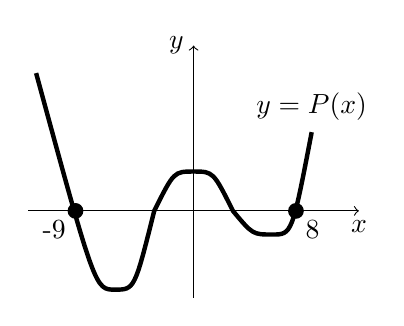
\begin{tikzpicture}

\draw[->] (-2.1, 0) -- (2.1,0) node[below] {$x$};
\draw[->] (0, -1.1) -- (0, 2.1) node[left] {$y$};

\draw[ultra thick] (-2,1.75) .. controls (-1.25, -1) and (-1.25, -1) .. (-1, -1) .. 
  controls (-0.75,-1) and (-0.75,-1) .. (-0.5, 0) ..
  controls (-0.25,0.5) and (-0.25,0.5) .. (0, 0.5) .. 
  controls (0.25,0.5) and (0.25,0.5) .. (0.5, 0) .. 
  controls (0.75,-0.3) and (0.75,-0.3) .. (1, -0.3) .. 
  controls (1.25,-0.3) and (1.25,-0.3) .. (1.5, 1) node[above] {$y = P(x)$};

\fill[black] (-1.5, 0) circle (1mm) node [below left] {-9};
\fill[black] (1.3, 0) circle (1mm) node [below right] {8};

\end{tikzpicture} \end{center}





\question \textbf{Bonus.} We assume $k \in \mathbb{R}$. Given that $f(x)=x^3+kx^2-2x+1$ and that when $f(x)$  is divided by $(x-k)$ the remainder is $k$, find the possible values of $k$. \hfill \emph{Work on the back.}

\vfill

\end{questions}

\begin{tcolorbox}

\textbf{Name of examiner:}

\begin{center}
\gradetable[h][questions]
\end{center}

\end{tcolorbox}


\end{document}